\section{Local Imitation Dynamics for Public Good Games}
\subsection{Outline}
This chapter investigates the linear PGG under imitation dynamics. Imitation dynamics come from the same family as replicator dynamics introduced in \eqref{rep}, with $\alpha = 0$. Hence $q_{i\to j} = \mathbbm{1}_{\{\pi_j>\pi_i\}}$. The tests from Chapter \ref{Chapter:Rep} are run for imitation dynamics, and the similarities and differences to imitation dynamics are noted. \\

\subsection{Results}
\FloatBarrier
\graphCap{ID_gtype_low.pdf}{0.7}{Comparing Graph Models: Imitation Dynamics. Trend for $r \in \{4.0, 4.25, 4.5, 4.75\}$. In each graph, the blue circles, orange stars, green crosses, and red pentagons correspond to the WS model, TAG model, BA model, and RRG model respectively.Only the BA graph model induces non-trivial cooperation.}{imitation_low} 
\FloatBarrier
\graphCap{ID_gtype_med.pdf}{0.7}{Comparing Graph Models: Imitation Dynamics. Trend for $r \in \{5.0, 5.25, 5.5, 5.75\}$. In each graph, the blue circles, orange stars, green crosses, and red pentagons correspond to the WS model, TAG model, BA model, and RRG model respectively. The BA model still induces the highest cooperation, and the RRG consistently induces the lowest.}{imitation_medium}
\FloatBarrier
\graphCap{ID_gtype_high.pdf}{0.7}{Comparing Graph Models: Imitation Dynamics. Trend for $r \in \{6,6.5,7,7.5\}$. In each graph, the blue circles, orange stars, green crosses, and red pentagons correspond to the WS model, TAG model, BA model, and RRG model respectively. The TAG model overtakes the BA model, while the RRG still fails to achieve non-zero cooperation. }{imitation_high}\FloatBarrier

Relative to replicator dynamics, less cooperation is observed for each graph model and parameter $r$. Furthermore, the \emph{re-ordering} effect noticed in Figure \ref{replicator_medium} and Figure \ref{replicator_high}, whereby the cooperation initially drops and then returns, is not observed to the same level. \\

For $r<6.25$, the order of the models, from most to least cooperation, is the BA model, then TAG, then WS, and finally the RRG. In fact, for $r<7$, the RRG model never achieves non-zero cooperation. A possible explanation is the faster switching rate of strategies. Under imitation dynamics, player $i$ randomly chooses a neighbour $j$, and then always switches if $\pi_j>\pi_i$. In comparison, under replicator dynamics, the probability of switching is proportional to the difference in payoff. Therefore $i$ does not always switch to $j$, even if $\pi_j>\pi_i$. For this reason, the environment may be able to \emph{re-order}, and spread cooperation further before it becomes extinct. \\

In the regime $r\geq 6.25$, the TAG model overtakes the BA model for higher cooperation. This phenomenon was also noticed under replicator dynamics in Figure \ref{replicator_medium}, but instead occurred at $r=5.25$. A possible explanation is the higher clustering coefficient for the TAG model. This allows groups of cooperation to form, which then spread further and induce higher cooperation. \\

For consistency, the same tests from Chapter \ref{Chapter:Rep} are reproduced under imitation dynamics. \\

\subsection{Isolating the Effect of Clustering Coefficient: Power Law Degree Size Distribution}

\FloatBarrier
\graphCap{ID_power_p_low.pdf}{0.7}{To test the effect of $C_\Delta$, the parameter $p$ in a PL graph was varied. In each graph, the blue circles, orange stars, green crosses, red pentagons, and purple squares correspond to $p\in\{0.1,0.2,0.3,0.4,0.5\}$ respectively. The observed trend is that higher $p$, and hence higher $C_\Delta$, leads to  higher cooperation.}{ID_power_p_low}
\FloatBarrier
\graphCap{ID_power_p_med.pdf}{0.7}{To test the effect of $C_\Delta$, the parameter $p$ in a PL graph was varied. In each graph, the blue circles, orange stars, green crosses, red pentagons, and purple squares correspond to $p \in \{0.1,0.2,0.3,0.4,0.5\}$ respectively. The trend is also observed here, with some minor discrepancies. For example, $p=0.4$ induces higher cooperation in a $r=5$ regime than $p=0.5$.}{ID_power_p_med} \FloatBarrier

The trend from Figure \ref{power_p_med} is reproduced here, namely that higher $p$, and hence higher $C_\Delta$, induces higher cooperation. This could be due to the higher clustering coefficient, or higher degree variance. Also note that the time to stability is much faster in these models than Figures \ref{power_p_low} and \ref{power_p_med}. This is because the probability of agent $i$ adopting agent $j$'s strategy, given $\pi_j > \pi_i$ is always 1 under imitation dynamics. Under replicator dynamics, this is not guaranteed and hence the rate at which strategies are changed is slower. \\


\subsection{Isolating the Effect of Clustering Coefficient: Constant Degree Size Distribution}

\graphCap{ID_graph_p_med.pdf}{0.7}{Effect of Rewiring $p$ in a WS model. In each graph, the blue circles, orange stars, green crosses, red pentagons, and purple squares correspond to $p \in \{0.1,0.2,0.3,0.4,0.5\}$ respectively. The trend indicates that higher $p$, and hence lower $C_\Delta$, leads to higher cooperation. }{ID_graph_p_med}\FloatBarrier
 


\graphCap{ID_graph_p_high.pdf}{0.7}{Effect of Rewiring $p$ in a WS model. In each graph, the blue circles, orange stars, green crosses, red pentagons, and purple squares correspond to $p \in \{0.1,0.2,0.3,0.4,0.5\}$ respectively. The observed trend is an increase in $p$, and hence a reduction in $C_\Delta$, leads to higher cooperation.}{ID_graph_p_high}
\FloatBarrier

 Similar to Figure \ref{graph_p_med}, the effect of high $p$ does not dominate until $r$ is past a certain threshold. The threshold is $5.75$ for replicator dynamics, and $6$ for imitation dynamics. This indicates the impediment to the spread of cooperation in a low $r$, high $p$ environment is not unique to replicator dynamics. \\
 
 In general, the trend observed in Figures \ref{graph_p_med} and \ref{graph_p_high} were replicated here. Higher variance in degree distribution leads to higher cooperation. However the time to equilibrium is much faster for imitation dynamics. \\
 
\subsection{The Effect of Mean Degree: RRG}

\graphCap{ID_graph_m_low_RRG.pdf}{0.8}{The effect of mean degree, RRG model. In each graph, the blue circles, orange stars, green crosses, red pentagons, and purple squares correspond to the mean degree $m \in \{4,6,8,10,12\}$ respectively. An increase in $m$ results in lower mean cooperation.  }{ID_graph_m_low} \FloatBarrier

\graphCap{ID_graph_m_med_RRG.pdf}{0.8}{The effect of mean degree, RRG model. In each graph, the blue circles, orange stars, green crosses, red pentagons, and purple squares correspond to the mean degree $m \in \{4,6,8,10,12\}$ respectively. An increase in $m$ results in lower mean cooperation.  }{ID_graph_m_med} \FloatBarrier



\graphCap{ID_graph_m_high_RRG.pdf}{0.8}{The effect of mean degree, RRG model. In each graph, the blue circles, orange stars, green crosses, red pentagons, and purple squares correspond to mean degree $m \in  \{4,6,8,10,12\}$ respectively. Once again, an increase in $m$ results in lower cooperation }{ID_graph_m_high} \FloatBarrier

It is evident that $r>m+1$ is required for full cooperation in the RRG model. It is also interesting  to constrast the trends corresponding to $m=4, r \to 5$, and $m=6, r \to 7$. As $r$ approaches $m+1$ for $m=4$, moderate cooperation is induced, however in the case $m=6$, all trials result in a full defection equilibrium. On the other hand, for $m = 6, r \to 7$ in Figure \ref{graph_m_med} and Figure \ref{graph_m_high}, some moderate cooperation is observed. This is a major difference between replicator and imitation dynamics. \\




\FloatBarrier
\graphCap{ID_graph_m_low_BA.pdf}{0.8}{The effect of mean degree, BA model. In each graph, the blue circles, orange stars, green crosses, red pentagons, and purple squares correspond to targeted mean degree $m = \{4,6,8,10,12\}$ respectively. For the BA model, an increase in $m$ also results in lower cooperation.}{ID_BA_graph_m_low}
\FloatBarrier
\graphCap{ID_graph_m_med_BA.pdf}{0.8}{The effect of mean degree, BA model. In each graph, the blue circles, orange stars, green crosses, red pentagons, and purple squares correspond to targeted mean degree $m = \{4,6,8,10,12\}$ respectively. For the BA model, an increase in $m$ results in lower cooperation.}{ID_BA_graph_m_med}
\FloatBarrier

\graphCap{ID_graph_m_high_BA.pdf}{0.8}{The effect of mean degree, BA model. In each graph, the blue circles, orange stars, green crosses, red pentagons, and purple squares correspond to targeted mean degree $m = \{4,6,8,10,12\}$ respectively. For the BA model, an increase in $m$ results in lower cooperation.}{ID_BA_graph_m_high}
\FloatBarrier

Firstly, note that the BA model generally reports higher cooperation than the RRG model for given $r,m$. This corresponds to previous trials. Under the BA model, some medium levels of cooperation are observed. This can be attributed to some realisations of the network inducing full cooperation. It is not shown, but the 2.5\% and 97.5\% quantiles were investigated for the BA and RRG models. In the case corresponding to $m=8, 4 = 4.25$, the 97.5\% quantile BA model was able to achieve full cooperation. This contrasts with $m=6, r = 6.75$, where the 97.5\% quantile realisation resulted in no contribution. The variance between realisations of a BA network is much higher, and this leads to reported average equilibria between 0 and 1. 

\subsection{Cooperation Level Within a Single Graph Instance: BA model } 


\FloatBarrier 
\begin{figure}[!h]
  \begin{subfigure}[b]{0.45\textwidth}
    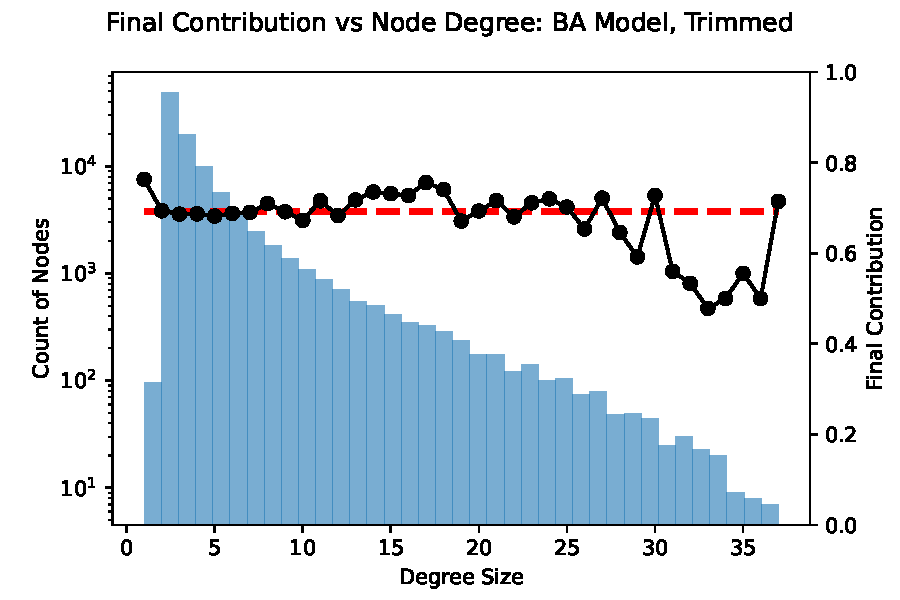
\includegraphics[width=1.1\textwidth]{images/ID_BA_node_groups_m_4_phi_4_trimmed.pdf}
    \caption{Final Cooperation by Degree, BA Model, Trimmed, for $m=4$, $r=4$.   }
    \label{ID_by_degree_m_4_phi_4}
  \end{subfigure}
  \hfill
  \begin{subfigure}[b]{0.45\textwidth}
    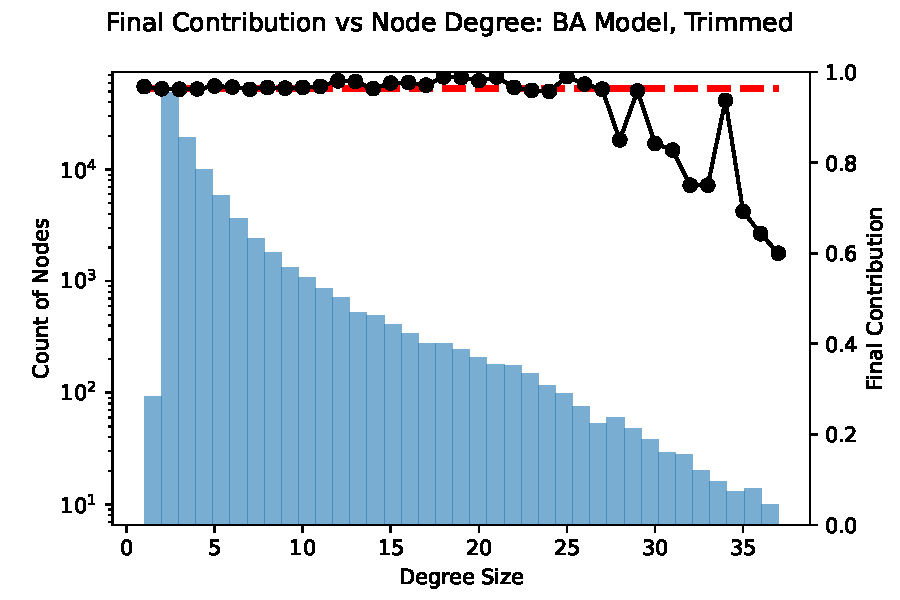
\includegraphics[width=1.1\textwidth]{images/ID_BA_node_groups_m_4_phi_6_trimmed.pdf}
    \caption{Final Cooperation by Degree, BA Model, Trimmed, for $m=4$, $r=6$. }
    \label{ID_by_degree_m_4_phi_6}
  \end{subfigure}
  \caption{The histogram, plotted on the left axis, shows the count of nodes with given degree. The black trend line is the mean cooperation for nodes of that degree, measured at the final step. Finally, the red line is the overall mean cooperation, also measured at the final step. Both plots indicate that higher node degrees contribute less than lower node degrees.} \label{ID_by_degree_m_4}
\end{figure} 
\FloatBarrier


\FloatBarrier 
\begin{figure}[!h]
  \begin{subfigure}[b]{0.45\textwidth}
    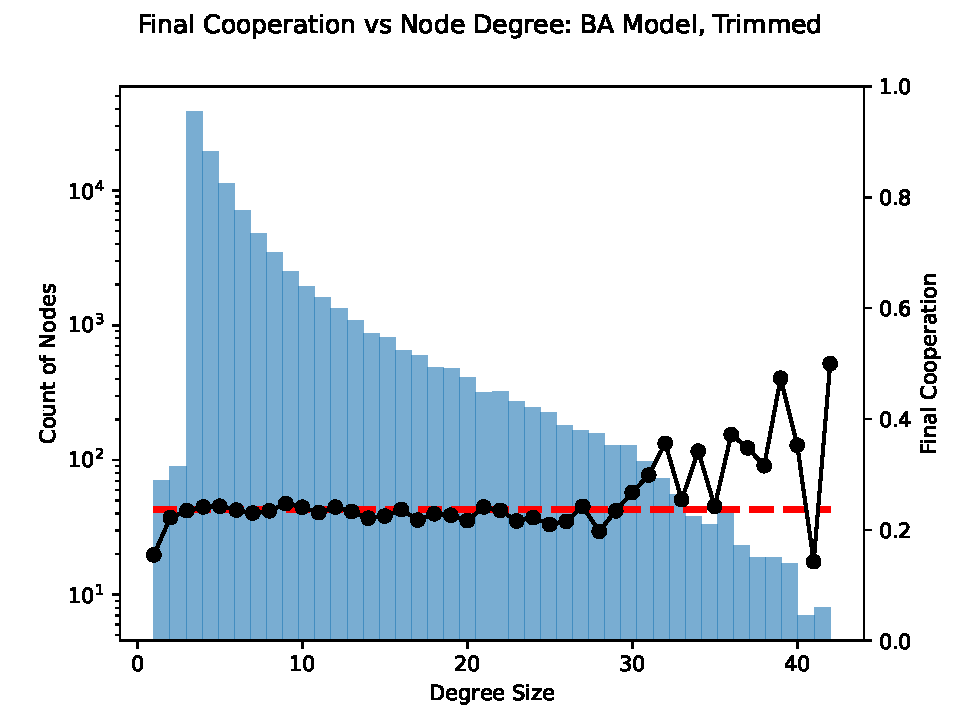
\includegraphics[width=1.1\textwidth]{images/Rep_BA_node_groups_m_6_phi_4_trimmed.pdf}
    \caption{Final Cooperation by Degree, BA Model, Trimmed, for $m=6$, $r=4$.   }
    \label{ID_by_degree_m_6_phi_4}
  \end{subfigure}
  \hfill
  \begin{subfigure}[b]{0.45\textwidth}
    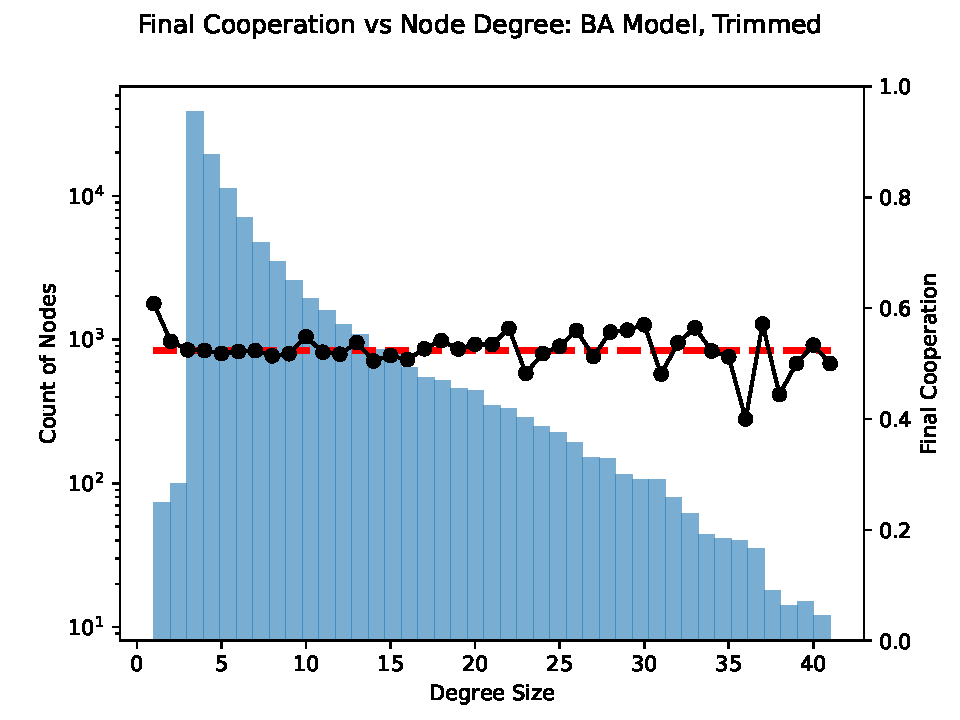
\includegraphics[width=1.1\textwidth]{images/ID_BA_node_groups_m_6_phi_6_trimmed.pdf}
    \caption{Final Cooperation by Degree, BA Model, Trimmed, for $m=6$, $r=6$. }
    \label{ID_by_degree_m_6_phi_6}
  \end{subfigure}
  \caption{The histogram, plotted on the left axis, shows the count of nodes with given degree. The black trend line is the mean cooperation for nodes of that degree, measured at the final step. Finally, the red line is the overall mean cooperation, also measured at the final step. Both plots indicate that higher node degrees contribute less than lower node degrees.} \label{ID_by_degree_m_6}
\end{figure} 
\FloatBarrier


\FloatBarrier 
\begin{figure}[!h]
  \begin{subfigure}[b]{0.45\textwidth}
    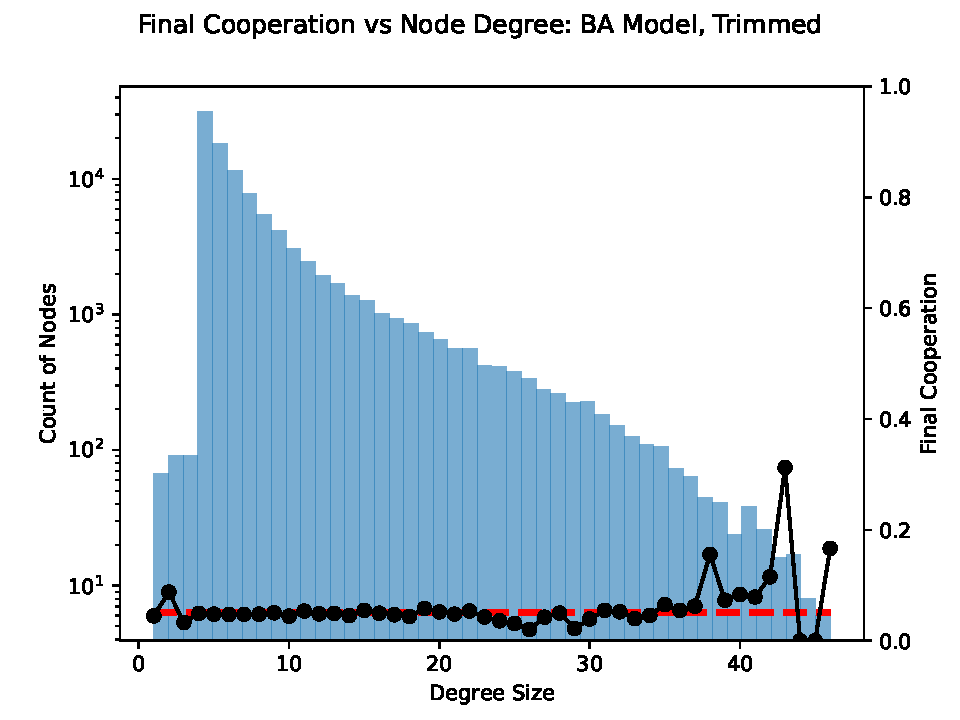
\includegraphics[width=1.1\textwidth]{images/Rep_BA_node_groups_m_8_phi_4_trimmed.pdf}
    \caption{Final Cooperation by Degree, BA Model, Trimmed, for $m=8$, $r=4$.   }
    \label{ID_by_degree_m_8_phi_4}
  \end{subfigure}
  \hfill
  \begin{subfigure}[b]{0.45\textwidth}
    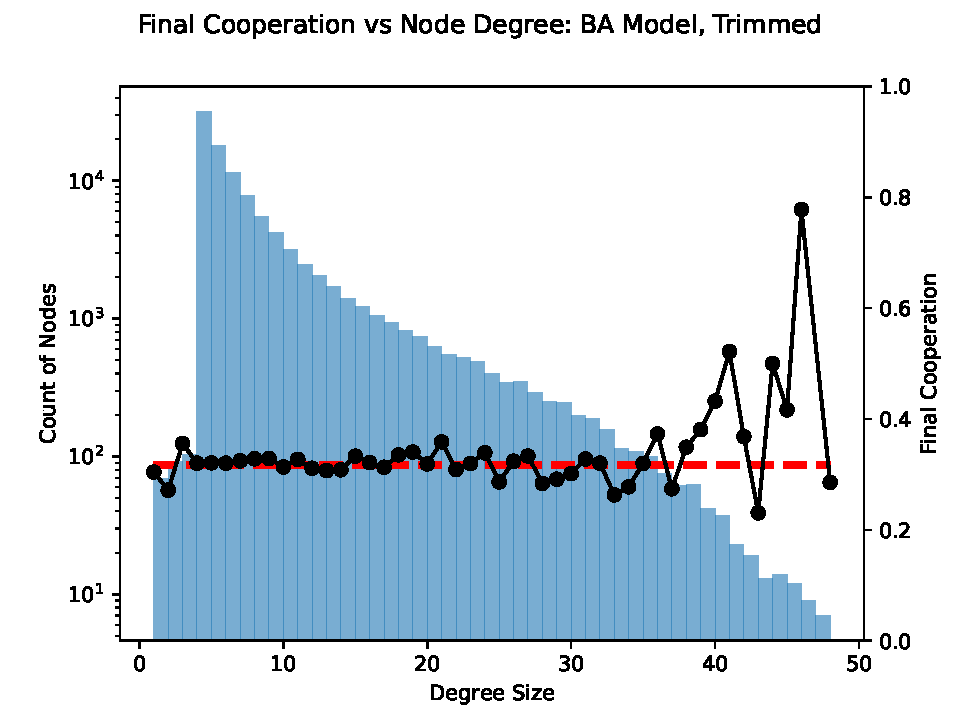
\includegraphics[width=1.1\textwidth]{images/Rep_BA_node_groups_m_8_phi_6_trimmed.pdf}
    \caption{Final Cooperation by Degree, BA Model, Trimmed, for $m=8$, $r=6$. }
    \label{ID_by_degree_m_8_phi_6}
  \end{subfigure}
  \caption{The histogram, plotted on the left axis, shows the count of nodes with given degree. The black trend line is the mean cooperation for nodes of that degree, measured at the final step. Finally, the red line is the overall mean cooperation, also measured at the final step. Both plots indicate that higher node degrees contribute less than lower node degrees.} \label{ID_by_degree_m_8}
\end{figure} 
\FloatBarrier

The trend in these graphs is very similar to that observed in Figure \ref{by_degree_m_4}, Figure \ref{by_degree_m_6}, and Figure \ref{by_degree_m_8}. The nodes with high degree are not as influenced as the low degree nodes, so contribute less in a high contribution environment and more in a low contribution environment. At this stage, there is no explanation for these observations.

\subsection{Differences Between Replicator and Imitation Dynamics}

Both replicator and imitation dynamics produced a similar ranking of graph models. The graph models with a power-law degree distribution, specifically the BA and TAG models, induced higher cooperation than the RRG and WS models. The RRG model never achieved non-zero cooperation under imitation dynamics, yet surpassed the WS model and achieved quite substantial cooperation under replicator dynamics. This is one of the major differences. \\

Another major difference is the level of maximum cooperation achieved. Two figures are replicated below, and show the cooperation level, as well as a $95\%$ confidence interval around the mean. \\

\FloatBarrier 
\begin{figure}[!h]
  \begin{subfigure}[b]{0.45\textwidth}
    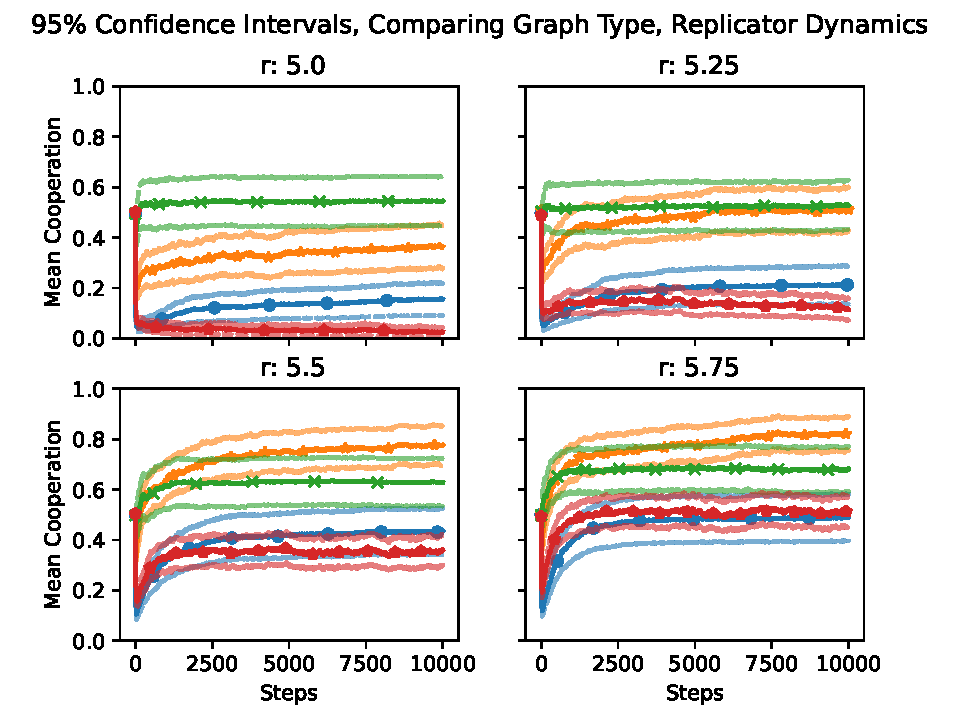
\includegraphics[width=1.1\textwidth]{images/Rep_gtype_med_CI.pdf}
    \caption{Comparing Graph Models, Replicator Dynamics.   }
    \label{rep_high_gtype_2}
  \end{subfigure}
  \hfill
  \begin{subfigure}[b]{0.45\textwidth}
    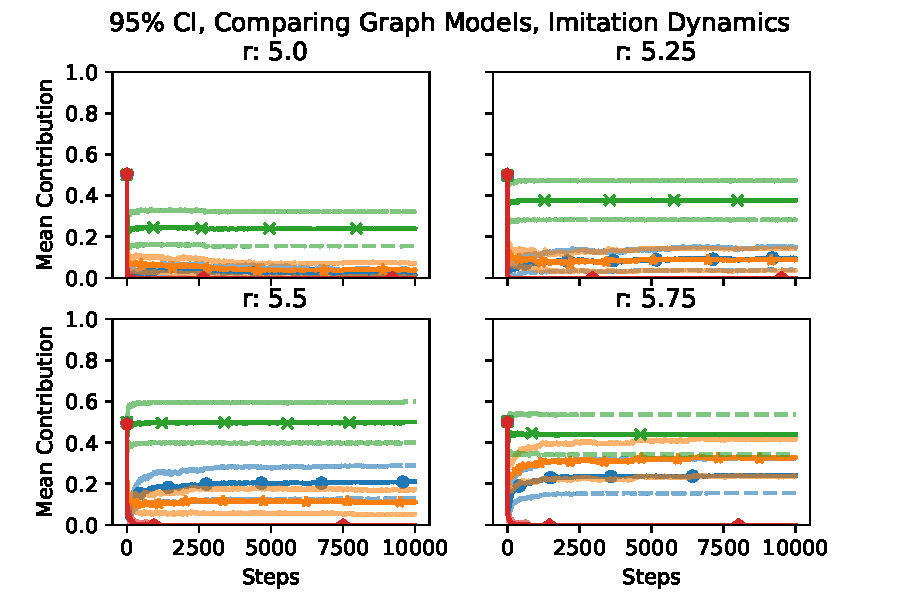
\includegraphics[width=1\textwidth]{images/ID_gtype_med_CI.pdf}
    \caption{Comparing Graph Models, Imitation Dynamics. }
    \label{ID_high_gtype_2}
  \end{subfigure}
  \caption{Replication of Figure  \ref{replicator_med} and Figure \ref{imitation_med} with confidence intervals. For every graph model, replicator dynamics induce higher cooperation. The width of the confidence intervals is quite similar between replicator and imitation dynamics. } \label{comparing_rep_ID_high}
\end{figure} 
\FloatBarrier

It is hard to examine the size of the confidence intervals visually, so Figure \ref{rep_dev} and \ref{id_dev} collate the variance of cooperation in the final timestep for each graph model. \\

\graphCap{Rep_dev_heatmap.pdf}{0.9}{Cap}{rep_dev}

\graphCap{ID_dev_heatmap.pdf}{0.9}{cap}{id_dev}


A difference between replicator and imitation dynamics is the time to equilibrium, particularly in the case where the equilibrium is low cooperation. The time to equilibrium in a complete graph model is discussed in Lemma \ref{connected}, and it is shown that replicator dynamics achieve equilibrium much slower. While the simulated graph models are not complete graphs, there is some merit to the conclusion. This is because the probability that an agent $i$ changes to the strategy of agent $j$, given $\pi_j>\pi_i$, is 1 for imitation dynamics, and varies between 0 and 1 for replicator dynamics. So the equilibrium in imitation dynamics can be achieved faster as agents always change to a more profitable strategy once they observe it. \\



Replicator and imitation dynamics showed similar results when varying the clustering parameter $p$ in a PL model and also the rewiring parameter $p$ in the WS model. Increasing variance, regardless of the effect on the clustering coefficient, generally increases cooperation. The same effect is observed when varying rewiring $p$ in a WS model. Equilibrium is achieved much faster under imitation dynamics, but higher equilibria are observed for replicator dynamics. 



\begin{table}[]
\begin{tabular}{|l|l|l|l|l|}
\hline
     & WS    & TAG   & BA    & RRG \\ \hline
4.0  & 0.0   & 0.097 & 0.338 & 0.0 \\ \hline
4.25 & 0.0   & 0.102 & 0.405 & 0.0 \\ \hline
4.5  & 0.0   & 0.103 & 0.394 & 0.0 \\ \hline
4.75 & 0.08  & 0.174 & 0.419 & 0.0 \\ \hline
5.0  & 0.084 & 0.174 & 0.428 & 0.0 \\ \hline
5.25 & 0.285 & 0.272 & 0.485 & 0.0 \\ \hline
5.5  & 0.409 & 0.303 & 0.503 & 0.0 \\ \hline
5.75 & 0.429 & 0.459 & 0.499 & 0.0 \\ \hline
6.0  & 0.465 & 0.493 & 0.495 & 0.0 \\ \hline
6.25 & 0.49  & 0.475 & 0.493 & 0.0 \\ \hline
6.5  & 0.502 & 0.456 & 0.445 & 0.0 \\ \hline
6.75 & 0.49  & 0.418 & 0.478 & 0.0 \\ \hline
\end{tabular}
\caption{Imitation Final Deviation}
\label{tab:ID_dev}
\end{table}

\begin{table}[]
\begin{tabular}{|l|l|l|l|l|}
\hline
     & WS    & TAG   & BA    & RRG   \\ \hline
4.0  & 0.015 & 0.031 & 0.404 & 0.0   \\ \hline
4.25 & 0.075 & 0.151 & 0.466 & 0.0   \\ \hline
4.5  & 0.174 & 0.231 & 0.484 & 0.0   \\ \hline
4.75 & 0.25  & 0.309 & 0.463 & 0.043 \\ \hline
5.0  & 0.328 & 0.439 & 0.496 & 0.099 \\ \hline
5.25 & 0.378 & 0.444 & 0.494 & 0.216 \\ \hline
5.5  & 0.465 & 0.391 & 0.481 & 0.312 \\ \hline
5.75 & 0.474 & 0.337 & 0.457 & 0.306 \\ \hline
6.0  & 0.485 & 0.313 & 0.437 & 0.237 \\ \hline
6.25 & 0.49  & 0.251 & 0.41  & 0.203 \\ \hline
6.5  & 0.465 & 0.156 & 0.391 & 0.177 \\ \hline
6.75 & 0.474 & 0.139 & 0.353 & 0.098 \\ \hline
\end{tabular}
\caption{Replicator Final Standard Deviation}
\label{tab:Rep_final}
\end{table}
\begin{itemize}
    \item Imitation dynamics moves a lot more often, as prob move given greater payoff is 1. This means goes to 0 faster, and potentially can't return
    \item Also means the diminishing return of defect in a defect environment is not punished
    \item Faster to equilibrium, as less \emph{waiting} for probabilities to hit
    \item Same ordering of graph models, but different switch time. I would hypothesise this is because it cares more about degree variance overall. 
    \item 
\end{itemize}
\subsection{Simple Results}
\newtheorem{remark1}[theorem]{Remark} \label{remark1}
\begin{remark1}
For a RRG, with $r>m+1$, the NE is full cooperation, however it is not necessarily achieved. This is because the defector is a drain on their neighbouring cooperators, and is unable to see a full contributor. 
\end{remark1}
\begin{proof}
Consider a lone defector in a RRG environment. Also assume that none of the neighbours of the defector are connected to each other. The defector's payoff, called $\pi_D$, is calculated as $m+1$ games with $m$ contributors, hence $$\pi_D = (m+1) \times \frac{mr}{m+1} = mr. $$ This defector only changes to cooperation if one of its neighbours has higher payoff. The payoff of a neighbour, denoted $\pi_C$, is the result of their hosted game, plus the defectors hosted game, plus $m-1$ games of full cooperation, hence $$\pi_C = \frac{mr}{m+1}+\frac{mr}{m+1} + (m-1) \frac{(m+1 )r}{m+1} - (m+1) = \frac{2mr}{m+1} +(m-1)r - (m+1) $$ 


The condition for the defector to change strategy is $\pi_C  - \pi_D>0$. Consider the case when this is true. \\
\begin{align*}
    \pi_C - \pi_D &= \frac{2mr}{m+1} +r(m-1) -(m+1)-mr\\
    &= \frac{2mr}{m+1} -(m+1+r)\\
    \frac{2mr}{m+1} -(m+1+r) &> 0\\
    \frac{2mr}{m+1} &>(m+1+r)\\
    mr &>(m+1)^2+r\\
    r&>\frac{(m+1)^2}{m-1}
\end{align*}
This is a stricter condition than the hypothesis $r>m+1$, so the defector may not necessarily change. However changing would be the right decision, as their payoff becomes that of a full cooperator, $\pi_{F}$, $$ \pi_F = (m+1)\frac{(m+1)r}{m+1} - (m+1) = (m+1)(r-1). $$ This payoff is greater than $\pi_D$ for $r>m+1$. Furthermore, this shows that full cooperation is a NE, as no player has a unilateral incentive to deviate from full cooperation. The defector is unable to see the benefits of full cooperation because all of their neighbours' profits are diminished by the defectors choice. \end{proof}

The remark \ref{remark1} does not imply that no defector could ever switch to cooperation in a RRG model with $r>m+1$. It is simple to contrive an example where a defector \emph{sees} a cooperator with higher profit. It simply requires that the defector is connected to a lot of other defectors, while the cooperator is supported by other cooperators. Furthermore, full cooperation may be achieved, because the strategy changes are synchronous. Multiple defectors may all decide to switch at the same time, avoiding the lone defector problem from \ref{remark1}. \\

Furthermore, the above analysis does not extend to other graph models, because of the strict assumption that each node has the same degree. In a BA model, the defector may be connected to a cooperator of high degree, with all their neighbours also cooperating. This changes the solution to $\pi_C - \pi_D>0$. \\
\FloatBarrier
\newtheorem{lemma_connected}[theorem]{Lemma} \label{connected}
\begin{lemma_connected}
For the linear public goods game played on a complete graph, then the only ESS is full defection, regardless of $n$ or $r$. This holds for replicator and imitation dynamics, however the time to equilibrium is less for imitation dynamics.  \end{lemma_connected}
\begin{proof}
Consider the payoff of a contributor on the complete graph, and hence playing $c_i = 1$, $$\pi_i(c_i = 1) = \frac{r n_c}{n} - n,  $$ where $n_c$ is the total number of contributors. On the other hand, the payoff of a defector, hence playing $c_i = 0$, is $$\pi_i(c_i = 0) = \frac{r n_c}{n}. $$ Regardless of parameters $n$ or $r$, the payoff for a defector is higher. Hence there is only flow of contributors becoming defectors, and the ESS is full defection. \\

Now consider the time to reach equilibrium. Call the probability that a given cooperator $i$ changes to defection in a given generation is $q_{n_c}$. Then  $$q_{n_c} = \mathbb P(c_{i,t+1} = 0 | c_{i,t} = 1) = \mathbb P (c_{i,t+1} = 0 | c_{i,t} =1, c_{\text{nbr}, t = 0})\mathbb P(c_{\text{nbr},t} = 0), $$ where $c_{\text{nbr},t}$ is the contribution of the randomly selected neighbour in the reproduction step. Each of these terms is calculable, so \\
\begin{align*}
    \mathbb P(c_{i,t+1} = 0 | c_{i,t} = 1) &= \frac{n-n_c}{n}\Bigg[ \frac{|\pi_{\text{nbr},t} - \pi_{i,t}|}{\Delta} \Bigg]^\alpha\\
    &= \frac{n-n_c}{n}\Bigg[ \frac{\tfrac{rn_c}{n} - \tfrac{rn_c}{n} +n}{\tfrac{rn_c}{n}} \Bigg]^\alpha\\
    &= \frac{n-n_c}{n}\Bigg[ \frac{1}{rn_c} \Bigg]^\alpha\\
\end{align*}
For replicator dynamics, the parameter $\alpha = 1$, so the probability of a given agent changing strategies is $ q_{n_c} = \frac{n-n_c}{n}\Bigg[ \frac{1}{rn_c} \Bigg]$. For imitation dynamics, $\alpha = 0$, and the probability becomes $q_{n_c} = \frac{n-n_c}{n}$. \\

Finally, we can compute the expected time to equilibrium. Make the assumption that the timesteps are continuous, and then the event that one of the contributors becomes a defector is a Poisson random variable, and the distribution of the time between events is an exponential random variable with parameter $q_{n_c}$. The distribution of the minimum of $n$ i.i.d exponential $q_{n_c}$ random variables is an exponential distribution with parameter $n_c q_{n_c}$. So the time for $n_c$ to decrease by 1, denoted $T_{{n_c},{n_{c-1}}}$, is an exponential random variable with parameter $n_c q_{n_c}$. Call $T_{n_c, 0}$ the time to equilibrium from the current level of cooperators $n_c$. 
\begin{align*}
    \mathbb E (T_{n_c, 0} | n_c = n_c) &= \sum_{i = n_c}^1 \mathbb E (T_{{i}, {i-1}}|n_c = i)\\
    &= \sum_{i = n_c}^1 \frac{1}{iq_i}\\
\end{align*}
For replicator dynamics, this evaluates to 
\begin{align*}
       \mathbb E (T_{n_c, 0} | n_c = n_c) &= \sum_{i = n_c}^1 \frac{nr}{(n-i)}. 
\end{align*}
For imitation dynamics, 
\begin{align*}
    \mathbb E (T_{n_c, 0} | n_c = n_c) &= \sum_{i = n_c}^1 \frac{n}{i(n-i)}. 
\end{align*}
It is evident that imitation dynamics achieves the equilibrium faster, as the respective $q_i$ is higher so there is faster rate of change from contribution to defection. It is also interesting to note that the time to equilibrium for imitation dynamics does not depend on the rate $r$. \\

\end{proof}


